\clearpage

\section {Results of the $\bar{\nu}_{\mu}$-disappearance analysis with the Run 5+6 dataset}
\label{sec:results}

%--------------------------------------------------------------------------------------
% Best-fit params & pulls
%--------------------------------------------------------------------------------------

\subsection {Best-fit oscillation parameters}
\label{sec:results_bestfit}

Two 3-flavour $\bar{\nu}_{\mu}$-disappearance fits were performed on the combined \TotalPot{} 
POT Run 5+6 dataset, using the method described in Sec.~\ref{sec:oscfit_method}.
In the first fit, the normal mass hierarchy was assumed, 
and $\sin^{2}\overline{\theta}_{23}$ and $|\overline{\Delta m}^{2}_{32}|$ were allowed to float, 
while, in the second fit, the inverted mass hierarchy was assumed 
and $\sin^{2}\overline{\theta}_{23}$ and $|\overline{\Delta m}^{2}_{31}|$ were allowed to float. 
In both fits, 
%$\sin^{2}\overline{\theta}_{23}$ and $|\overline{\Delta m}^{2}_{32}|$ and 
all \NSyst{} systematic parameters considered 
in this analysis were allowed to float. 

The reconstructed energy distribution of the Run 5+6 single $\mu$-like ring \TotalPot{} POT dataset is
shown in figure~\ref{fig:results_data_spectrum:normal} along with the best-fit energy spectrum assuming
the normal mass hierarchy. The same Run 5+6 data spectrum is also shown with the best-fit energy spectrum assuming
the inverted mass hierarchy in figure~\ref{fig:results_data_spectrum:inverted}.
A summary is given of the best-fit oscillation parameters, $\chi^{2}$ and p-values and the observed and 
expected numbers of events in SuperK in table~\ref{tab:data_fits:best_fit_values}.

Two sets of comparative best-fit spectra are also included, which use a coarser binning in reconstructed energy.
The bin edges used are \{0.0, 0.4, 0.7, 1.0, 1.5, 2.0, 3.0, 4.0, 5.0, 30.0 GeV\}.
Figures~\ref{fig:results_data_spectrum:normal:numode} and~\ref{fig:results_data_spectrum:inverted:numode}
show a comparison between the best-fit spectrum from this analysis and the spectrum given by the
T2K run 1-4 joint fit result.
Figures~\ref{fig:results_data_spectrum:normal:groups} and~\ref{fig:results_data_spectrum:inverted:groups}
show the VALOR spectra compared to the other oscillation groups.

\begin{figure*}[htb]
  \begin{minipage}[t]{0.96\linewidth}
    \center
    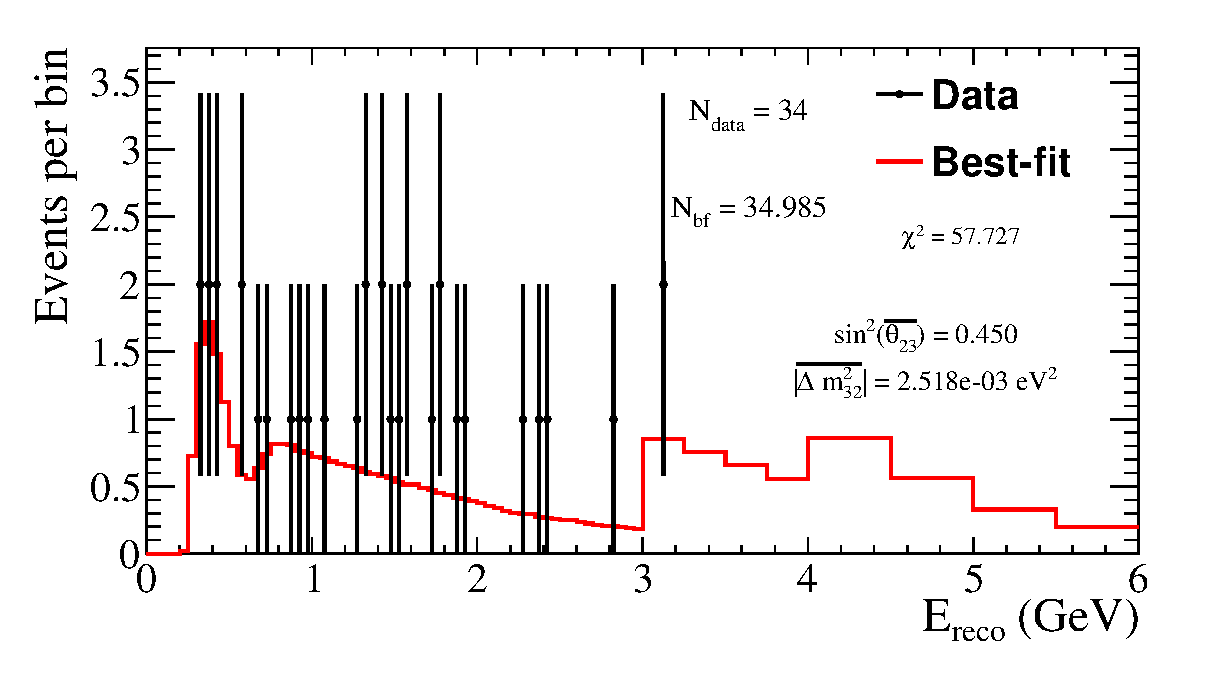
\includegraphics[width=36pc]{./images/data_fit/normal_spectrum_0.eps}
    \caption {
      The Run 5+6 single $\mu$-like ring \TotalPot{} POT dataset and the best-fit spectrum.
      The normal mass hierarchy is assumed.
      Note that total number of events per bin is shown, without taking into account bin width.
    }
    \label{fig:results_data_spectrum:normal}
  \end{minipage}
  \vfill
  \begin{minipage}[t]{0.96\linewidth}
    \center
    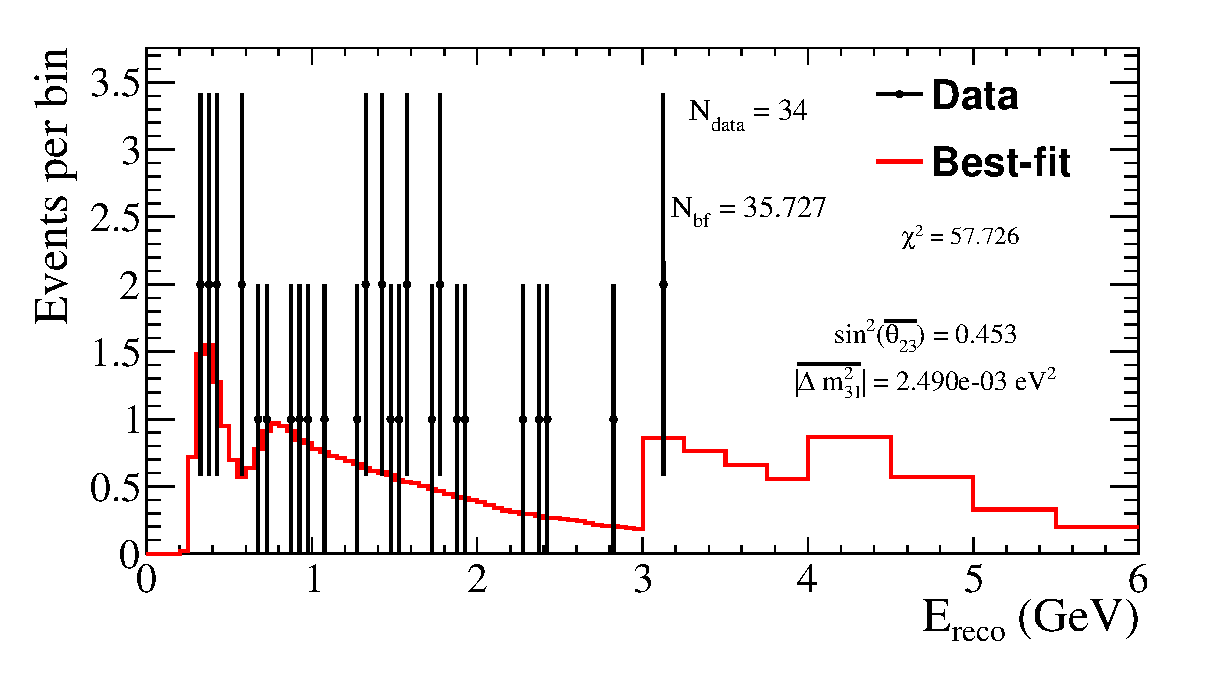
\includegraphics[width=36pc]{./images/data_fit/inverted_spectrum_0.eps}
    \caption {
      The Run 5+6 single $\mu$-like ring \TotalPot{} POT dataset and the best-fit spectrum.
      The inverted mass hierarchy is assumed.
      Note that total number of events per bin is shown, without taking into account bin width.
    }
    \label{fig:results_data_spectrum:inverted}
  \end{minipage}
\end{figure*}


\begin{figure*}[htb]
  \begin{minipage}[t]{0.96\linewidth}
    \center
    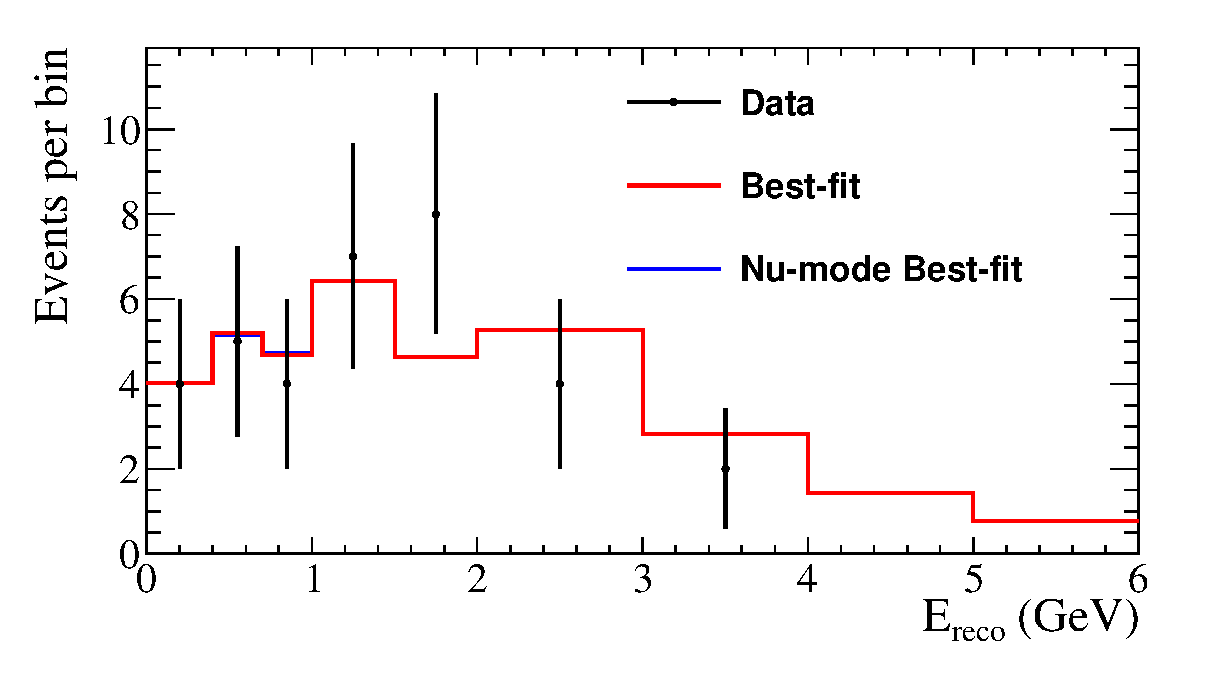
\includegraphics[width=36pc]{./images/data_fit/normal_spectrum_withnumode.eps}
    \caption {
      The Run 5+6 single $\mu$-like ring \TotalPot{} POT dataset and the best-fit spectrum.
      The binning is coarser than that used in the actual analysis (0.0, 0.4, 0.7, 1.0, 1.5, 2.0, 3.0, 4.0, 5.0, 30.0 GeV)
      and event counts are shown per bin. The VALOR normal mass hierarchy result is shown, and is compared with the best-fit 
      spectrum from the $\bar{\nu}_{\mu}$ dataset fixing \emph{all} the $\nu$ and $\bar{\nu}$ oscillation parameters to the T2K best-fit
      values from the Run 1-4 joint analysis as shown in table~\ref{tab:osc_params_fixed_values_reactor}, while still profiling the systematics.
    }
    \label{fig:results_data_spectrum:normal:numode}
  \end{minipage}
  \vfill
  \begin{minipage}[t]{0.96\linewidth}
    \center
    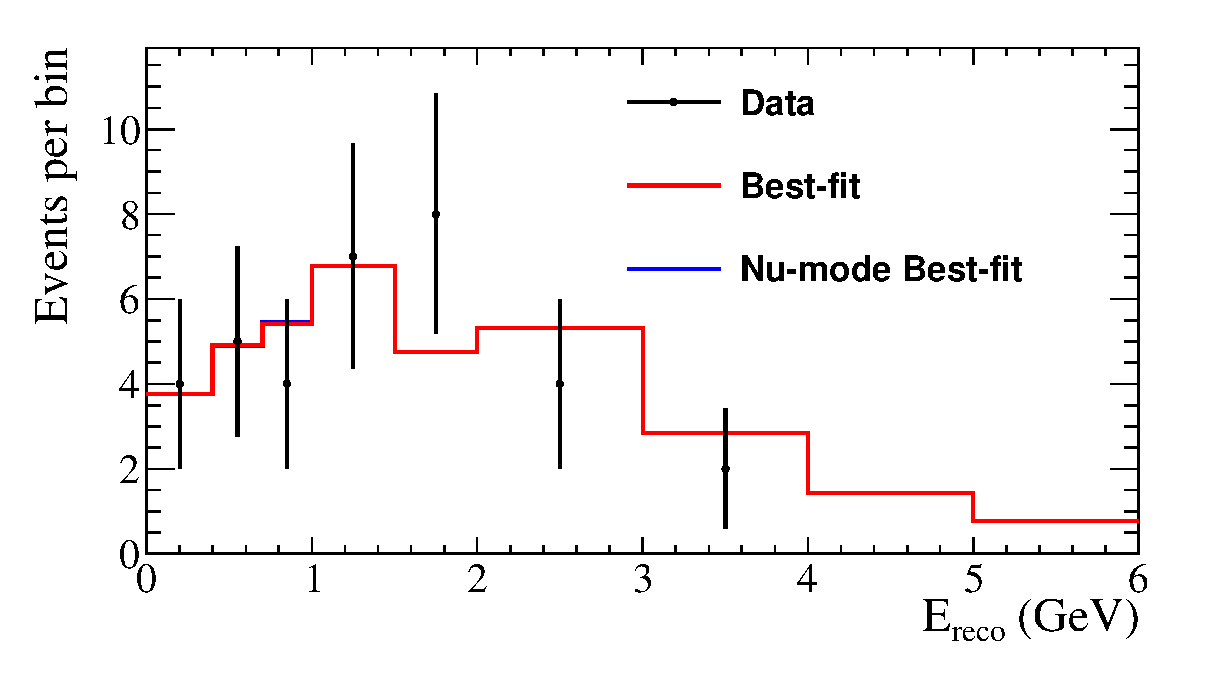
\includegraphics[width=36pc]{./images/data_fit/inverted_spectrum_withnumode.eps}
    \caption {
      The Run 5+6 single $\mu$-like ring \TotalPot{} POT dataset and the best-fit spectrum.
      The binning is coarser than that used in the actual analysis (0.0, 0.4, 0.7, 1.0, 1.5, 2.0, 3.0, 4.0, 5.0, 30.0 GeV)
      and event counts are shown per bin. The VALOR inverted mass hierarchy result is shown, and is compared with the best-fit
      spectrum from the $\bar{\nu}_{\mu}$ dataset fixing \emph{all} the $\nu$ and $\bar{\nu}$ oscillation parameters to the T2K best-fit
      values from the Run 1-4 joint analysis as shown in table~\ref{tab:osc_params_fixed_values_reactor}, while still profiling the systematics.
    }
    \label{fig:results_data_spectrum:inverted:numode}
  \end{minipage}
\end{figure*}

\begin{figure*}[htb]
  \begin{minipage}[t]{0.96\linewidth}
    \center
    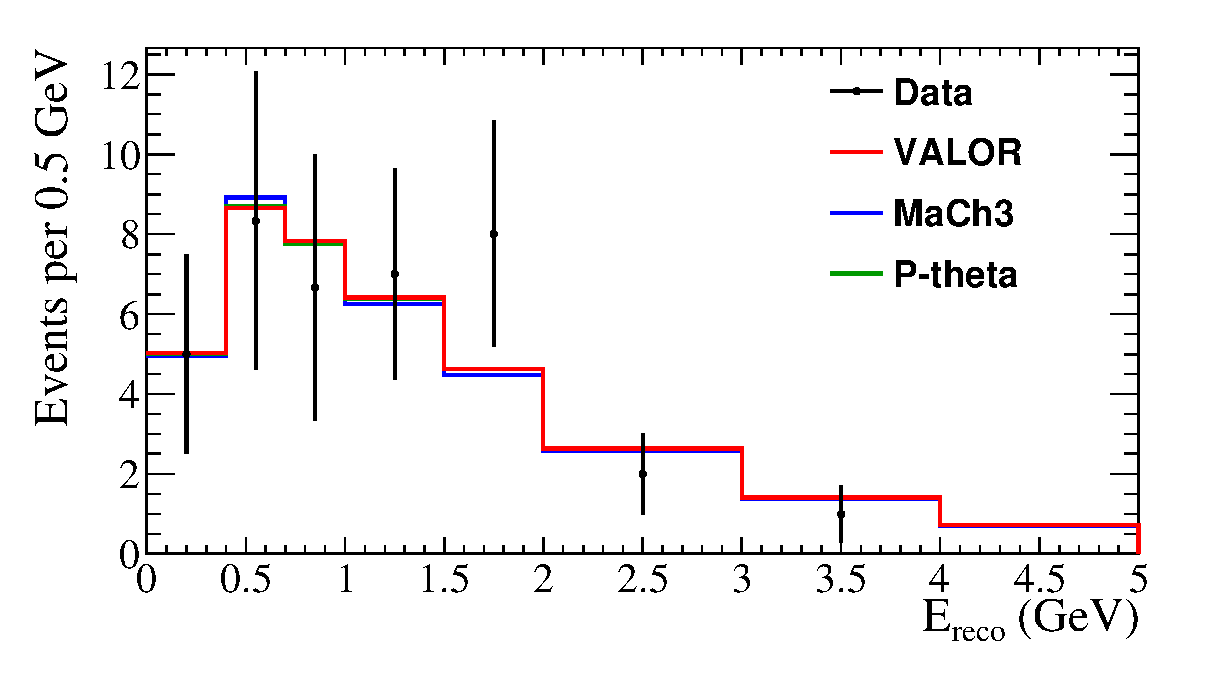
\includegraphics[width=36pc]{./images/data_fit/normal_coarse_spectrum_groups_per_energy.eps}
    \caption {
      The Run 5+6 single $\mu$-like ring \TotalPot{} POT dataset and the best-fit spectrum.
      This plot is more coarsely binned than the actual analysis and event counts are shown per unit energy.
      The VALOR normal mass hierarchy result is shown, compared to the other oscillation groups.
    }
    \label{fig:results_data_spectrum:normal:groups}
  \end{minipage}
  \vfill
  \begin{minipage}[t]{0.96\linewidth}
    \center
    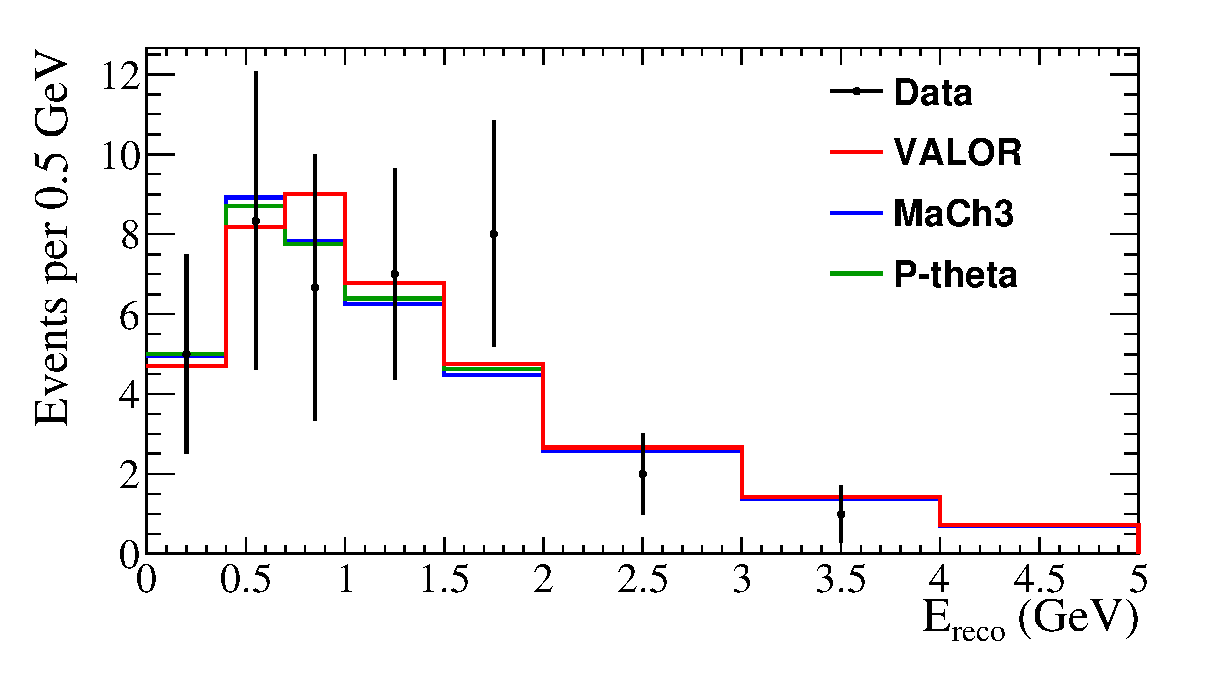
\includegraphics[width=36pc]{./images/data_fit/inverted_coarse_spectrum_groups_per_energy.eps}
    \caption {
      The Run 5+6 single $\mu$-like ring \TotalPot{} POT dataset and the best-fit spectrum.
      This plot is more coarsely binned than the actual analysis and event counts are shown per unit energy.
      The VALOR inverted mass hierarchy result is shown, compared to the other oscillation groups.
    }
    \label{fig:results_data_spectrum:inverted:groups}
  \end{minipage}
\end{figure*}



%...........................................................
%
% Table summarizing best-fit results
%
\begin{table}[htb]
\centering
\begin{tabular}{| l | l | c | c | c  c | c | c |}
\hline
Analysis & Run period & $\sin^{2}\overline{\theta}_{23}$ & $|\overline{\Delta m}^{2}_{32}|$/$|\overline{\Delta m}^{2}_{31}|$ & N$_{obs}$ & N$_{exp}$ & $\chi^2_{bf} / NDOF$ & p-value \\
\hline
2015 3-flavour Normal   & Run 5+6 & \BestFitMixingNormal &  \BestFitDmsqNormal 
& \NskObserved & \NskExpectedNormal & \BestFitNormalChisq & \PValueNormal \\
2015 3-flavour Inverted   & Run 5+6 & \BestFitMixingInverted &  \BestFitDmsqInverted 
& \NskObserved & \NskExpectedInverted & \BestFitInvertedChisq & \PValueInverted \\
\hline
\end{tabular}
\caption{
  Summary of best-fit parameters from the fits of the combined Run 5+6 dataset.
  The quoted best-fit $\chi^2$ values ($\chi^2_{bf}$) were computed from Eq.~\ref{eq:chisquare} in Sec.~\ref{sec:oscfit_method}.
  using the reconstructed energy binning scheme given in Sec.~\ref{sec:mc_templates:template_binning}.
  The table also shows the p-values obtained from the goodness-of-fit test described in Sec.~\ref{sec:gof_test}
  for all fits.
}
\label{tab:data_fits:best_fit_values}
\end{table}

\clearpage


\subsection {Goodness-of-fit tests}
\label{sec:results_gof}

Goodness-of-fit tests were performed for the fits of the real data as described 
in Sec.~\ref{sec:gof_test}, %\ 4.2 of Ref. \cite{OurRun123DisappAnalysis3Flavour},
and the results are shown in figures \ref {fig:results_data_goodness:normal} and 
\ref{fig:results_data_goodness:inverted}.
The p-values from these tests show that the fits are plausible for both mass hierarchies. 

%..................................
%
% Chisq_{gof} distributions
% 

\begin{figure*}[htb]
  \centering{
    \begin{minipage}[t]{0.9\linewidth}
      \center
      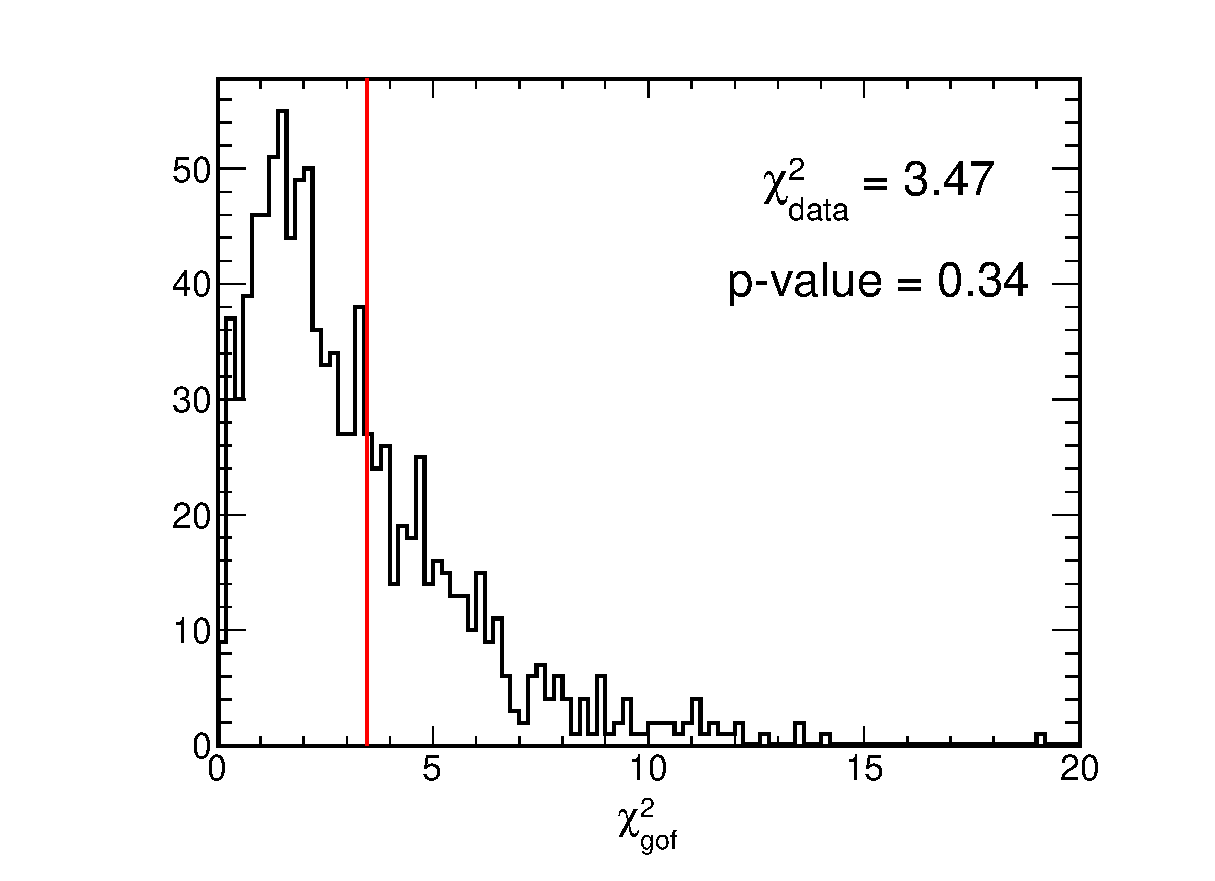
\includegraphics[width=24pc]{./images/data_fit/gof_t2kdata_4.011E20_statsyst_NH.eps}
      \caption {
        Distribution of $\chi^2_{gof}$, the goodness-of-fit (gof) $\chi^2$, from 1k toy MC experiments
        whose true input values are the best-fit oscillation parameters from the fit of the real data
        ($\sin^{2}\overline{\theta}_{23}$ = \BestFitMixingNormal, $|\overline{\Delta m}^{2}_{32}|$ = \BestFitDmsqNormal{} eV$^{2}$/c$^{4}$). 
        Systematic variations and statistical fluctuations are applied to the toy datasets, and all \NSyst{} systematic 
        parameters are included in the fits. 
        The toy experiments are generated for \TotalPot{} POT and the normal mass hierarchy is assumed.
        The $\chi^2$ value from the fit of the real data assuming the normal mass hierarchy (with all 
        \NSyst{} systematic parameters included in the fit) is shown as a red line.
      }
      \label{fig:results_data_goodness:normal}
    \end{minipage}
    \vfill
    \vspace{0.5cm}
    \begin{minipage}[t]{0.9\linewidth}

      \center
      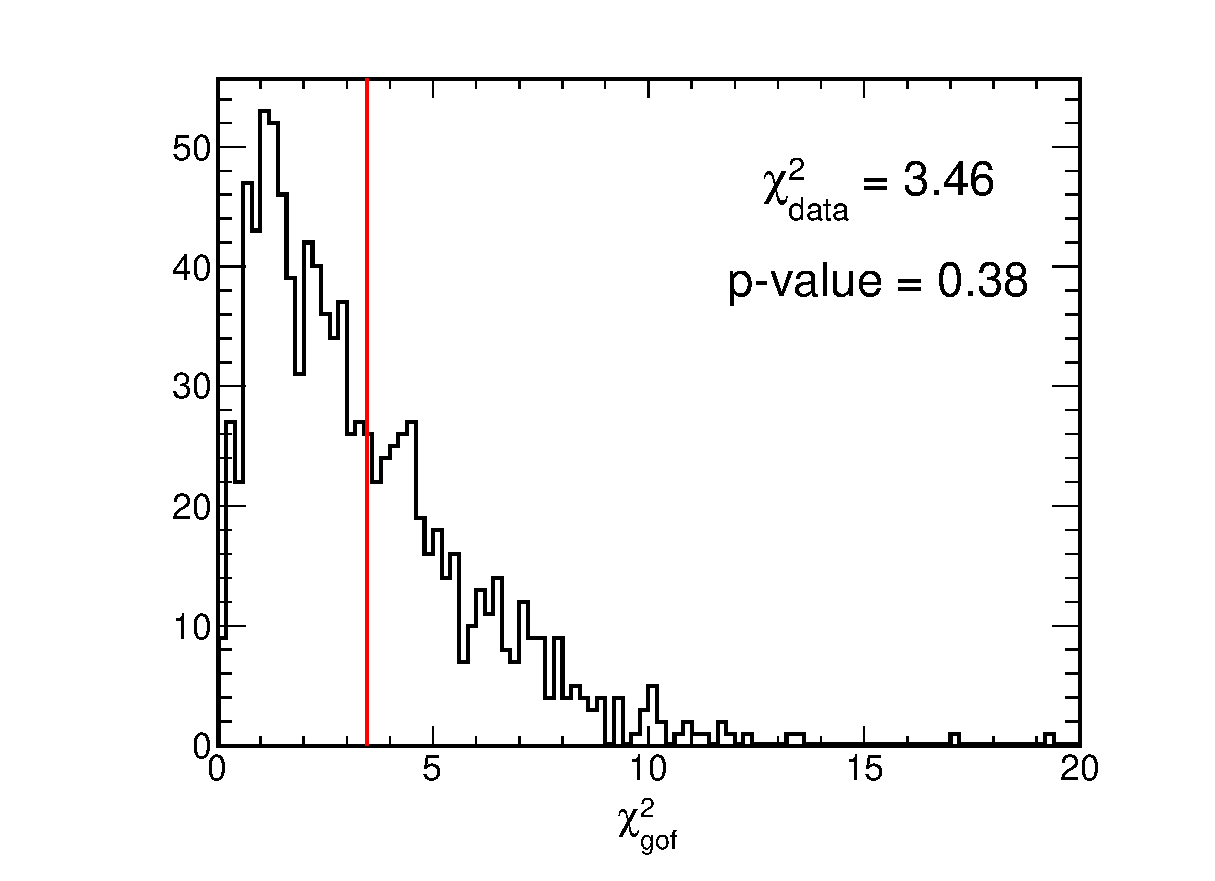
\includegraphics[width=24pc]{./images/data_fit/gof_t2kdata_4.011E20_statsyst_IH.eps}
      \caption {
        Distribution of $\chi^2_{gof}$, the goodness-of-fit (gof) $\chi^2$, from 1k toy MC experiments
        whose true input values are the best-fit oscillation parameters from the fit of the real data
        ($\sin^{2}\overline{\theta}_{23}$ = \BestFitMixingInverted, $|\overline{\Delta m}^{2}_{31}|$ = \BestFitDmsqInverted eV$^{2}$/c$^{4}$).
        Systematic variations and statistical fluctuations are applied to the toy datasets, and all \NSyst{} systematic
        parameters are included in the fits.
        The toy experiments are generated for \TotalPot{} POT and the inverted mass hierarchy is assumed.
        The $\chi^2$ value from the fit of the real data assuming the inverted mass hierarchy (with all \NSyst{} systematic 
        parameters included in the fit) is shown as a red line.
      }
      \label{fig:results_data_goodness:inverted}
    \end{minipage}
  }
\end{figure*}

\clearpage

\subsection {$\Delta\chi^2$ surfaces and confidence regions}
\label{sec:results_dchisq_contours}


$\Delta\chi^2$ surfaces from the fits of the combined Run 5+6 dataset are shown in figure~\ref{fig:results_data_chisq:normal} for 
the normal mass hierarchy and in figure~\ref{fig:results_data_chisq:inverted} for the inverted mass hierarchy.
The 68\% and 90\% allowed regions are shown using the constant-$\Delta\chi^2$ method in figures~\ref{fig:results_data_stat_vs_syst_nh} 
-~\ref{fig:results_data_asimov_contour_ih}: the first of these figures shows a comparison of the stat+syst confidence contour with 
the stat-only contour, and figures~\ref{fig:results_data_asimov_contour_nh_our_bf} and~\ref{fig:results_data_asimov_contour_nh_our_bf} show comparisons 
between the allowed regions from the fits of the combined Run 5+6 dataset with those from the fits of the Asimov dataset. 
These Asimov contours were produced at the best-fit oscillation parameter values from
this fit for $\sinsqb$ and $\dmsqb$, with other values fixed at values from
the T2K run 1-4 joint fit with reactor constraint, which
can be seen in table~\ref{tab:osc_params_fixed_values_reactor}.

Alternative Asimov contours produced using the input values to this analysis
can be seen in Appendix~\ref{app:asimov_fit_results}/

%...........................................................
% 
% \Delta\chisquare surfaces 
%
\begin{figure*}[htb]
  \begin{minipage}[t]{0.96\linewidth}
    \center
    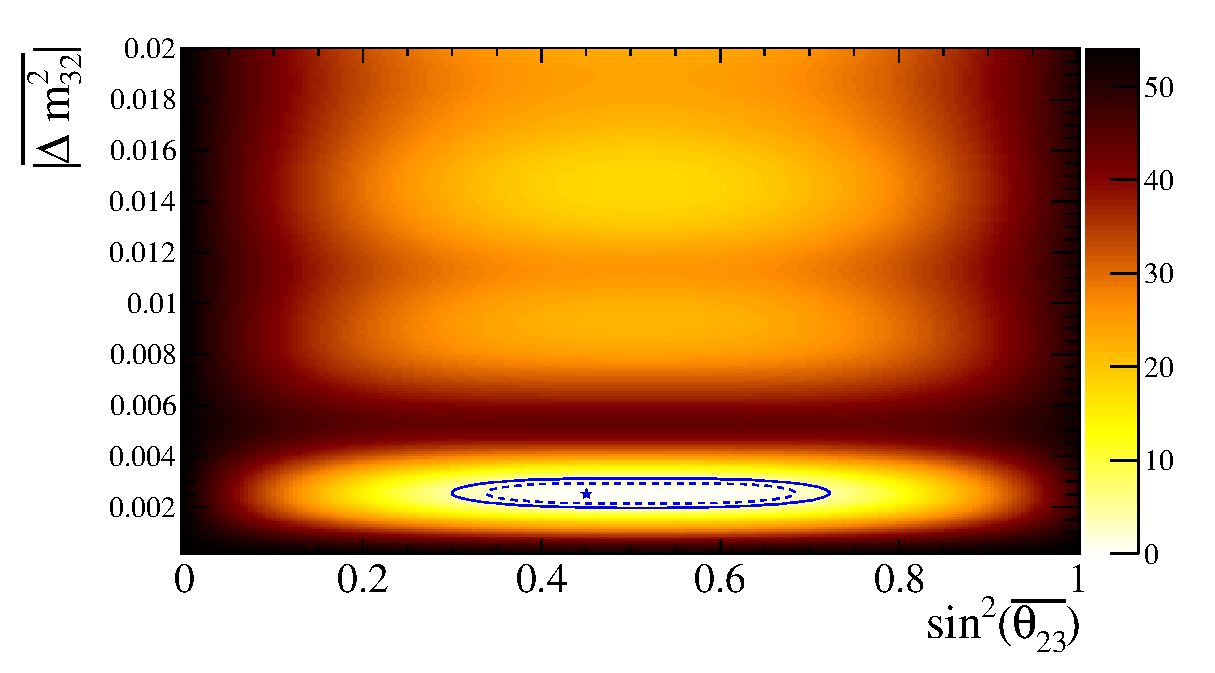
\includegraphics[width=0.9\textwidth]{./images/data_fit/realdata_with_reactor_values_nh.eps}
    \caption {
      $\Delta\chi^2$ surface from the fit of the \TotalPot{} POT run 5+6 dataset.
      The normal mass hierarchy is assumed.
      68\% and 90\% confidence contours are shown.
    }
    \label{fig:results_data_chisq:normal}
  \end{minipage}
  \vfill
  \begin{minipage}[t]{0.96\linewidth}
    \center
    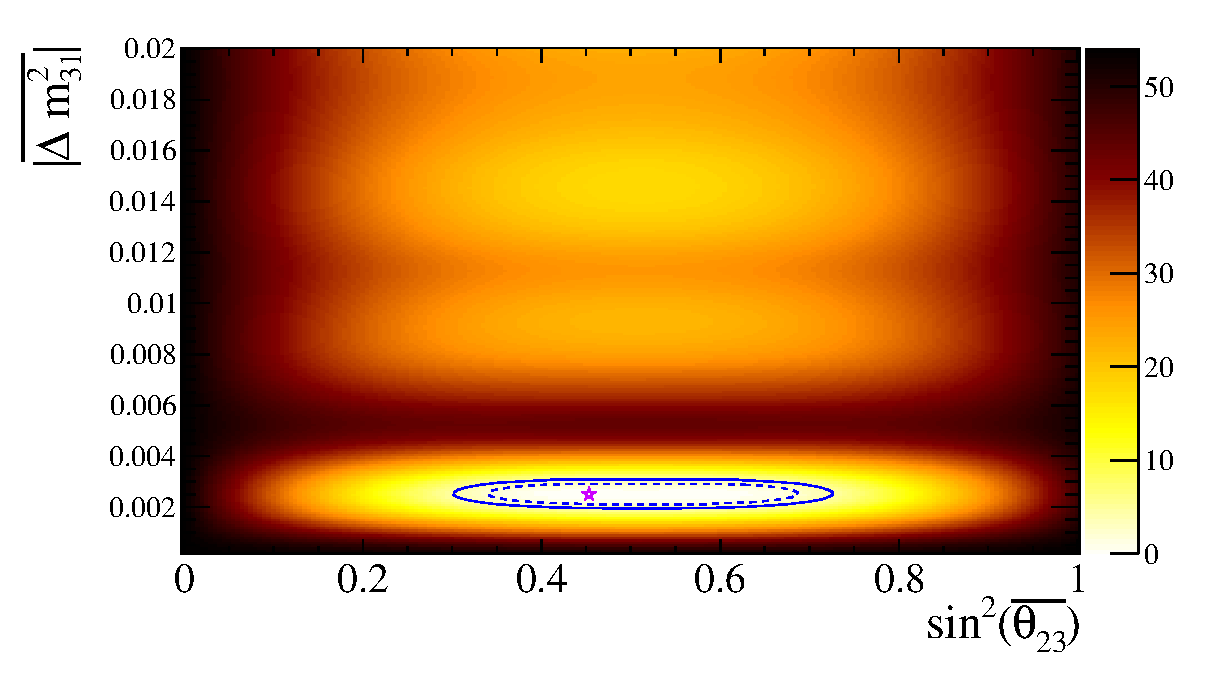
\includegraphics[width=0.9\textwidth]{./images/data_fit/realdata_with_reactor_values_ih.eps}
    \caption {
      $\Delta\chi^2$ surface from the fit of the \TotalPot{} POT Run 5+6 dataset.
      The inverted mass hierarchy is assumed.
      68\% and 90\% confidence contours are shown.
    }
    \label{fig:results_data_chisq:inverted}
  \end{minipage}
\end{figure*}

\clearpage

%...........................................................
%
% Const-dchi^2 contours 
%

\clearpage

\begin{figure*}[htb]
\center
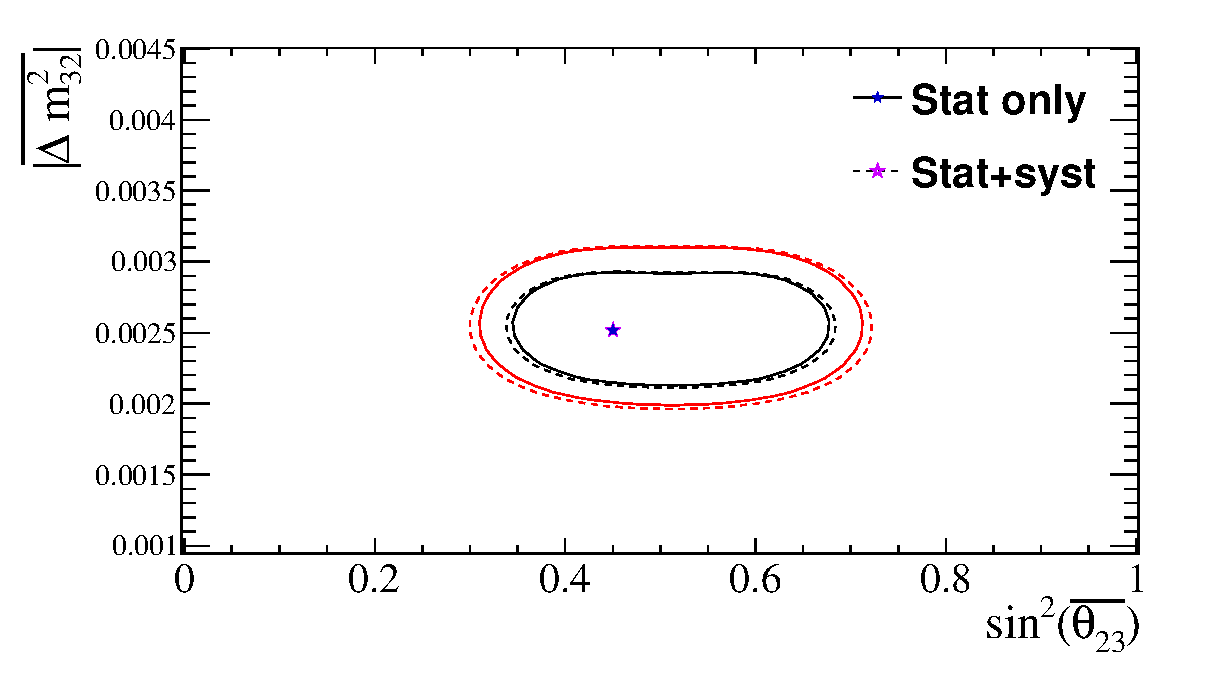
\includegraphics[width=0.9\textwidth]{./images/data_fit/stat_vs_syst_bestfit_zoomed_nh.eps}
\caption {
  68\% and 90\% CL allowed regions,
  constructed with the constant-$\Delta\chi^{2}$ method,
  from the fit to the Run 5+6 dataset.
  A comparison is shown between the full stat+syst contour
  and the contour with the systematic parameters fixed at their best-fit values.
  It can be seen that the fit is statistically limited.
  The normal hierarchy is assumed.
}
\label{fig:results_data_stat_vs_syst_nh}
\end{figure*}

\begin{figure*}[htb]
\center
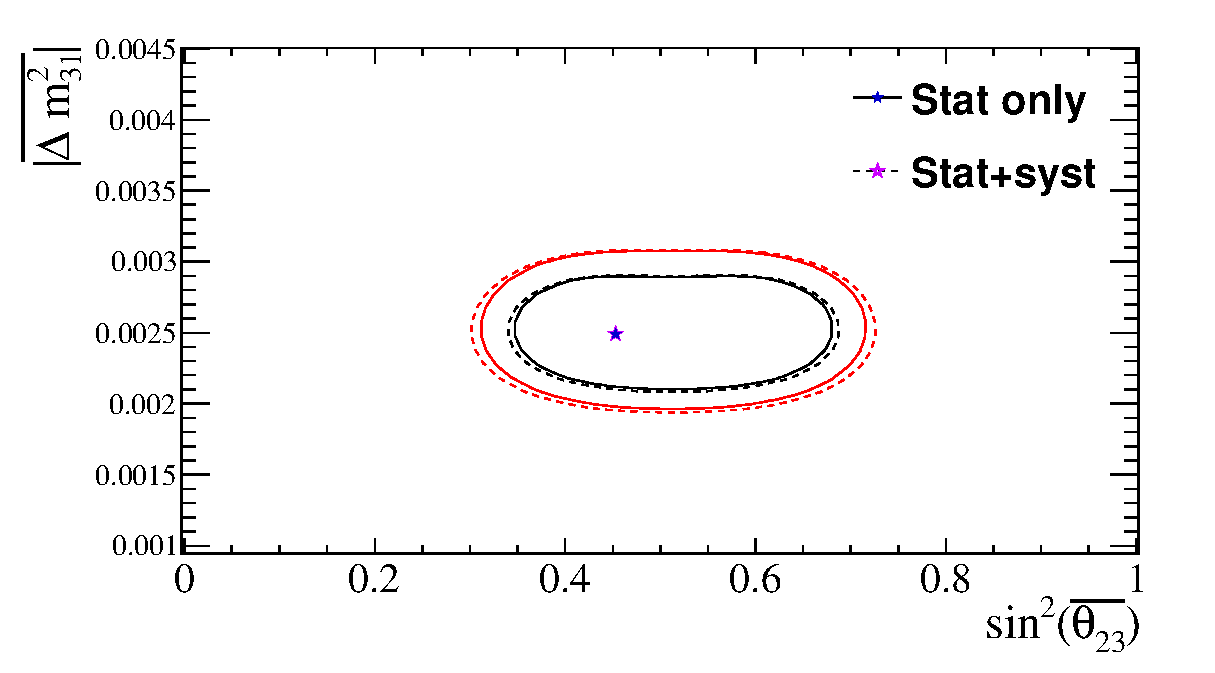
\includegraphics[width=0.9\textwidth]{./images/data_fit/stat_vs_syst_bestfit_zoomed_ih.eps}
\caption {
  68\% and 90\% CL allowed regions,
  constructed with the constant-$\Delta\chi^{2}$ method,
  from the fit to the Run 5+6 dataset.
  A comparison is shown between the full stat+syst contour
  and the contour with the systematic parameters fixed at their best-fit values.
  It can be seen that the fit is statistically limited.
  The inverted hierarchy is assumed.
}
\label{fig:results_data_stat_vs_syst_ih}
\end{figure*}


% Asimov dataset fit at the T2K data fit result

\begin{figure*}[htb]
\center
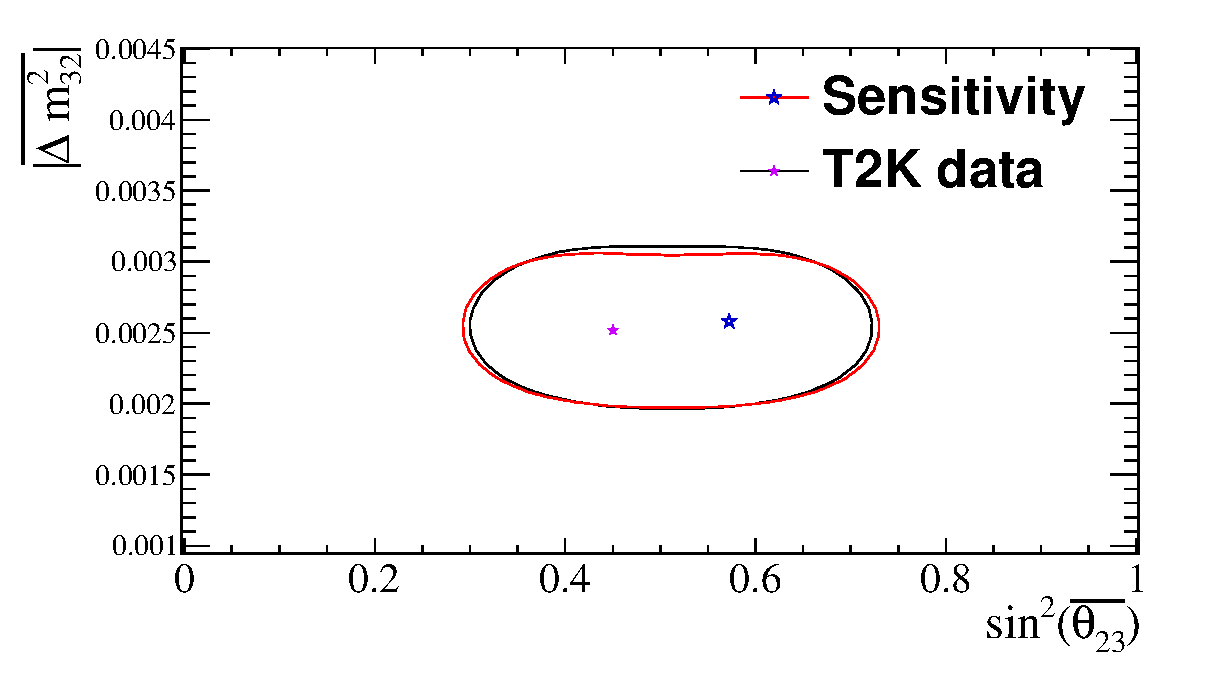
\includegraphics[height=0.35\textheight]{./images/asimov_fit/realdata_vs_asimov_our_bf_zoomed_nh.eps}
\caption {
  68\% and 90\% CL allowed regions,
  constructed with the constant-$\Delta\chi^{2}$ method,
  from the fit to the Run 5+6 dataset, 
  with the effects of statistical fluctuations and postfit systematic variations being included. 
  These contours compare a fit to the Asimov dataset with the fit to the real data.
  The normal hierarchy is assumed, and the data best-fit values of
  $\sinsqb = $ \BestFitMixingNormal{} and 
  $\dmsqb = $ \BestFitDmsqNormal{} are used.
  Other oscillation parameters are fixed at their values from the T2K
  run 1-4 joint fit with reactor constraint (table~\ref{tab:osc_params_fixed_values_reactor}).
}
\label{fig:results_data_asimov_contour_nh_our_bf}
\end{figure*}
\begin{figure*}[htb]
\center
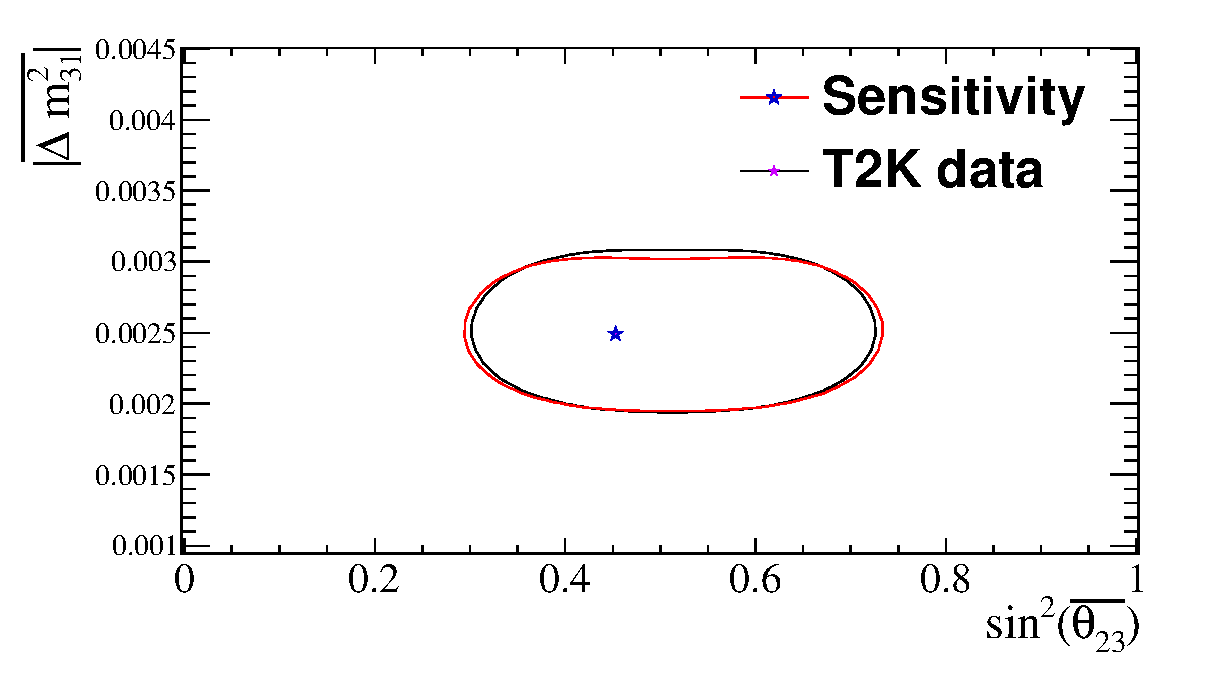
\includegraphics[height=0.35\textheight]{./images/asimov_fit/realdata_vs_asimov_our_bf_zoomed_ih.eps}
\caption {
  68\% and 90\% CL allowed regions,
  constructed with the constant-$\Delta\chi^{2}$ method,
  from the fit to Run 5+6 dataset, 
  with the effects of statistical fluctuations and postfit systematic variations being included. 
  These contours compare a fit to the Asimov dataset with the fit to the real data.
  The normal hierarchy is assumed, and the data best-fit values of
  $\sinsqb = $ \BestFitMixingInverted{} and 
  $\dmsqbih = $ \BestFitDmsqInverted{} are used.
  Other oscillation parameters are fixed at their values from the T2K
  run 1-4 joint fit with reactor constraint (table~\ref{tab:osc_params_fixed_values_reactor}).
}
\label{fig:results_data_asimov_contour_ih_our_bf}
\end{figure*}


%~ \begin{figure*}[htb]
%~ \center
%~ \includegraphics[width=36pc]{./images/data_fit/numubarDisappearance_data_wiRC_compareValorPTheta_extrazoomed_no2d.eps}
%~ \caption {
  %~ Overlayed contours for the three oscillation groups,
  %~ constructed with the constant-$\Delta\chi^{2}$ method,
  %~ from the fit to real data.
%~ }
%~ \label{fig:results_data_contour}
%~ \end{figure*}

%--------------------------------------------------------------------------------------
% Best-fit spectra
%--------------------------------------------------------------------------------------

%\subsection {Best-fit single-ring $\mu$-like reconstructed energy spectra}
%\label{sec:results_bestfit_spectra}

%--------------------------------------------------------------------------------------
% Contours
%--------------------------------------------------------------------------------------

\clearpage

%\subsection {Confidence regions}
%\label{sec:results_contours}

%The first step in constructing confidence contours in the 2-dimensional $\sin^{2}\overline{\theta_{23}}$ - $|\overline{\overline{\Delta m^{2}_{32}}}|$ or 
%$\sin^{2}\overline{\theta_{23}}$ - $|\overline{\overline{\Delta m^{2}_{31}}}|$
%oscillation parameter space is to construct the $\Delta\chi^2$ surface from the fit of the data.
%The oscillation parameter space is divided into a rectangular grid of width
%{\color{red} $\sin^{2}\overline{\theta_{23}}$ = 0.0025, $|\overline{\overline{\Delta m^{2}_{32}}|}$ 
%or $|\overline{\overline{\Delta m^{2}_{31}}}|$ = 0.025$\times$10$^{-3}$ eV$^{2}$/c$^{4}$,  }
%with a grid point at the centre of each rectangle. For each 
%mass hierarchy, two separate fits are made of 
%the data at each grid point: in one fit, the values of $\sin^{2}\overline{\theta_{23}}$ and $|\overline{\Delta m^{2}_{32}}|$ or $|\overline{\Delta m^{2}_{31}}|$ 
%%are fixed to the true values of the grid point and the \NSyst{} systematic parameters are allowed to float, 
%while, in the other fit, $\sin^{2}\overline{\theta_{23}}$, $|\overline{\Delta m^{2}_{32}}|$ or $|\overline{\Delta m^{2}_{31}}|$,  and the systematic parameters 
%are allowed to float. $\Delta\chi^2$ is then calculated as the 
%difference between the minimum values of $\chi^{2}$ from the two fits ($\chi^{2}$ is defined in Eq.\
%\ref{eq:chisquare} in Sec.~\ref{sec:oscfit_method}).

%These 2-dimensional $\Delta\chi^2$ surfaces from the fits of the Run 5+6 dataset are shown in
%Figs.~\ref{fig:results_data1234_chisq:normal} and~\ref{fig:results_data1234_chisq:inverted}
%as a function of $\sin^{2}\overline{\theta_{23}}$ and $|\overline{\Delta m^{2}_{32}}|$ or $|\overline{\Delta m^{2}_{31}}|$,
%for the normal and inverted mass hierarchies respectively.
%For comparison, the corresponding $\Delta\chi^2$ surfaces from the fits of the Run 5 and Run 6
%datasets are shown for the normal mass hierarchy 
%in Figs.~\ref{fig:results_data123_chisq} and~\ref{fig:results_data4_chisq} respectively.
%The same $\Delta\chi^2$ range is used in all colour plots to allow comparison.

%Confidence regions were constructed in the 2-dimensional parameter space $\sin^{2}\overline{\theta_{23}}$ and $|\overline{\Delta m^{2}_{32}}|$ or $|\overline{\Delta m^{2}_{31}}|$
%using the constant-$\Delta\chi^2$ method described in Sec.~\ref{sec:contour_construction} from the
%fits of the Run 5+6, Run 5 and Run 6 datasets.
%The 68\% and 90\% CL regions are shown
%in Figs.~\ref{fig:results_data1234_contour:normal} and~\ref{fig:results_data1234_contour:inverted}
%for the normal and inverted mass hierarchies respectively.
%The corresponding constant-$\Delta\chi^2$ contours for the Run 5 and Run 6 datasets are shown
%in Figs.~\ref{fig:results_data123_contour} and~\ref{fig:results_data4_contour} respectively.

%~ \begin{figure*}[htb]
%~ \center
%~ \includegraphics[width=36pc]{./images/data_fit/realdata_vs_asimov_zoomed_nh_data.eps}
%~ \caption {
  %~ 68\% CL and 90\% CL allowed regions, 
  %~ constructed with the constant-$\Delta\chi^{2}$ method,
  %~ from the fit of the Asimov dataset, 
  %~ with the effects of statistical fluctuations and postfit systematic variations being included. 
  %~ The data fit result contours have been overlayed here.
  %~ The normal mass hierarchy is assumed.
%~ }
%~ \label{fig:results_asimov_data_contour_nh}
%~ \end{figure*}
%~ 
%~ \begin{figure*}[htb]
%~ \center
%~ \includegraphics[width=36pc]{./images/data_fit/realdata_vs_asimov_zoomed_ih_data.eps}
%~ \caption {
  %~ 68\% CL and 90\% CL allowed regions, 
  %~ constructed with the constant-$\Delta\chi^{2}$ method,
  %~ from the fit of the Asimov dataset, 
  %~ with the effects of statistical fluctuations and postfit systematic variations being included. 
  %~ The data fit result contours have been overlayed here.
  %~ The inverted mass hierarchy is assumed.
%~ }
%~ \label{fig:results_asimov_data_contour_ih}
%~ \end{figure*}

$\Delta \chi^{2}$ surfaces and confidence intervals are shown for each of $\sin^2 \overline{\theta}_{23}$ 
and $\overline{\Delta m}^{2}_{32}$ separately in figures~\ref{fig:results_data_1d_mixing23}
and~\ref{fig:results_data_1d_dmsq} respectively. These figures were made using separate fits of the Run 
5+6 dataset in which the oscillation parameter not shown was profiled.
Similar fits were performed where this parameter was profiled without a penalty term, and these
gave extremely similar results.


\begin{figure*}[htb]
\center
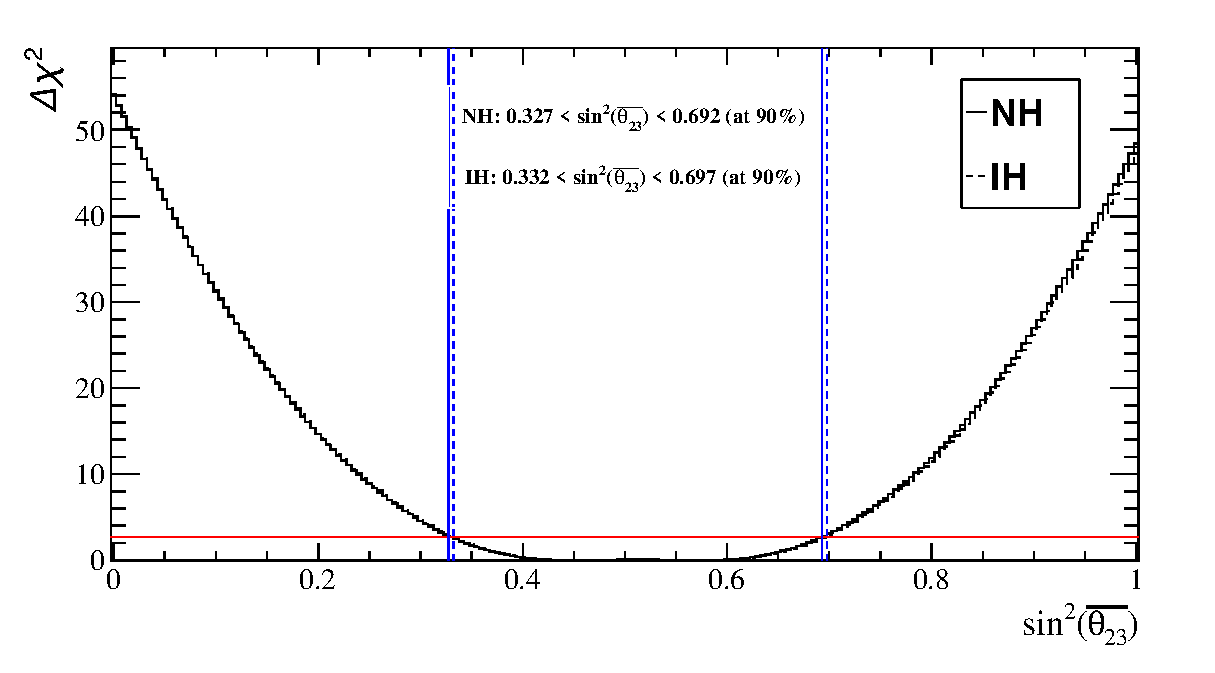
\includegraphics[width=0.8\textwidth]{./images/data_fit/conf_1d_free_mixing23.eps}
%~ 
\includegraphics[width=0.8\textwidth]{./images/missing_plot.eps}
\caption {
  Plots of 1D $\Delta\chi^{2}$ for $\sin^2 \overline{\theta}_{23}$ with $\overline{\Delta m}^{2}_{32}$ (normal hierarchy) 
  or $\overline{\Delta m}^{2}_{31}$ (inverted hierarchy) being profiled. These are from the fit of the \TotalPot real data
  with the effects of statistical fluctuations and postfit systematic variations being included. 
  Using the constant-$\Delta\chi^{2}$ method,
  the 1D 90\% CL allowed intervals are 0.357 $<$ $\sin^2 \overline{\theta}_{23}$ $<$ 0.662 (normal hierarchy) and 
  0.357 $<$ $\sin^2 \overline{\theta}_{23}$ $<$ 0.667 (inverted hierarchy).
}
\label{fig:results_data_1d_mixing23}
\end{figure*}

\begin{figure*}[htb]
\center
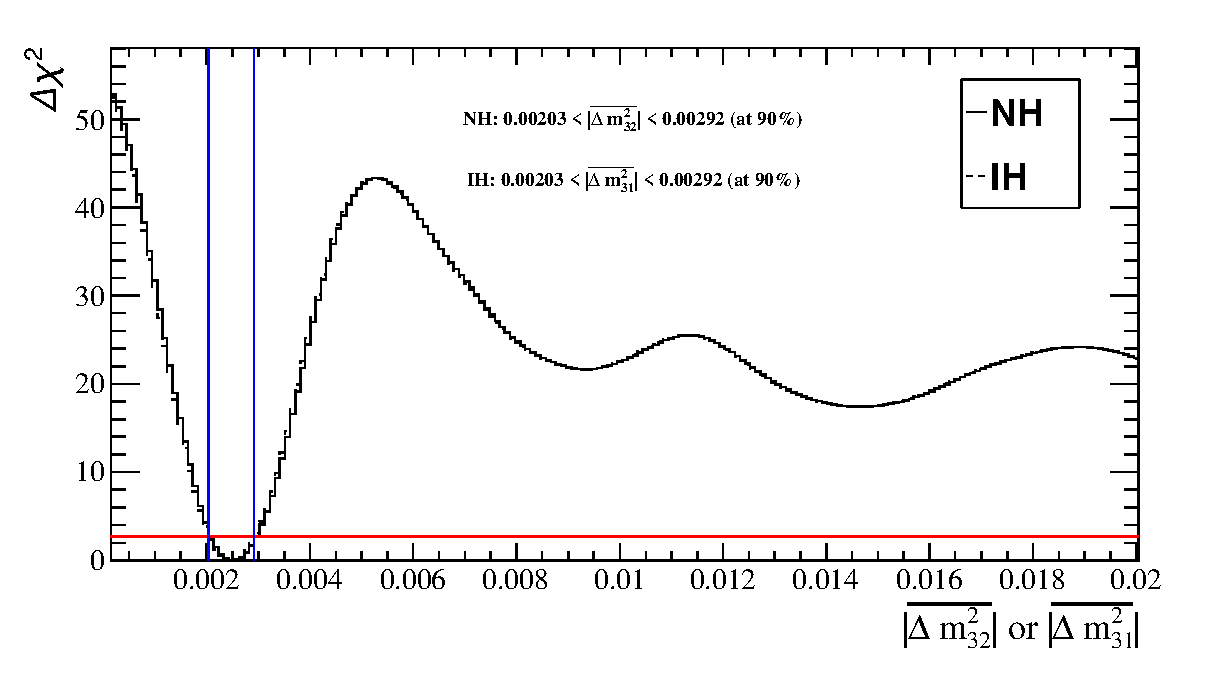
\includegraphics[width=0.8\textwidth]{./images/data_fit/conf_1d_free_dmsq.eps}
\caption {
  Plots of 1D $\Delta\chi^{2}$ for $\overline{\Delta m}^{2}_{32}$ (normal hierarchy) and $\overline{\Delta m}^{2}_{31}$ 
  (inverted hierarchy), with $\sin^2 \overline{\theta}_{23}$ being profiled. These are from the fit of the \TotalPot real data
  with the effects of statistical fluctuations and postfit systematic variations being included.
  Using the constant-$\Delta\chi^{2}$ method, 
  the 1D 90\% CL allowed intervals are 1.93$\times$10$^{-3}$eV$^{2}$/c$^{4}$ $<$ $\overline{\Delta m}^{2}_{32}$ $<$ 
  2.72$\times$10$^{-3}$eV$^{2}$/c$^{4}$ (normal hierarchy) and 1.93$\times$10$^{-3}$eV$^{2}$/c$^{4}$ $<$ 
  $\overline{\Delta m}^{2}_{31}$ $<$ 2.72$\times$10$^{-3}$eV$^{2}$/c$^{4}$ (inverted hierarchy).
}
\label{fig:results_data_1d_dmsq}
\end{figure*}



\clearpage

%--------------------------------------------------------------------------------------
% Contour comparisons
%--------------------------------------------------------------------------------------

\subsection {Comparisons of confidence regions}
\label{sec:results_contour_comparisons}

Figure~\ref{fig:results_data_contour_groups} shows a comparison between the VALOR result,
and the other T2K oscillation analysis groups. These analyses appear highly consistent.

In figure~\ref{fig:results_data_contour_minos}, we show a comparison between the 90\% CL allowed regions 
from the fits of the combined Run 5+6 dataset using the constant-$\Delta\chi^{2}$ method and a recent result from MINOS.

Previous versions of this note were released with \MarchPot POT,
and the expected increase in sensitivity with the current \TotalPot dataset
can be seen in figures~\ref{fig:results_asimov_changing_pot_nh} and~\ref{fig:results_asimov_changing_pot_ih}.
The difference between the previous data fit results and the current \TotalPot{}
data fit results can be seen in figures~\ref{fig:results_data_changing_pot_nh}
and~\ref{fig:results_data_changing_pot_ih}. Note that due to the best-fit
point moving away from maximal disappearance between the two fits, the
increased statistics do not usefully reduce the size of the contour.

Finally, we have produced a comparison with the official Run 1-4 T2K neutrino-mode fit result for the normal mass hierarchy, which is shown in 
figure~\ref{fig:results_data_contour_kdi}. The distribution of $\chi^2$ from 3k toy MC experiments whose true input values of 
$\sin^{2}\overline{\theta}_{23}$ and $|\overline{\Delta m}^{2}_{32}|$ are equal to the best-fit values of the equivalent parameters 
for the normal mass hierarchy from the official T2K Run 1-4 result in neutrino beam mode is shown in 
figure~\ref{fig:chisq_data_numode_bestfit_NH}. The value of $\chi^2$ from a fit of the Run 5-6 antineutrino beam mode data made 
while fixing $\sin^{2}\overline{\theta}_{23}$ and $|\overline{\Delta m}^{2}_{32}|$ to those same Run 1-4 best-fit values is 57.8. 
Given a null hypothesis of the neutrino-mode best-fit parameters, the p-value for the antineutrino beam mode data being 
as different or more different from the Run 1-4 neutrino-mode data than the actual Run 5-6 data is \PValueNuModeComp. It is a quantitative 
measure of the difference between the neutrino-mode and antineutrino-mode datasets. It means that the results of the Run 1-4 neutrino beam mode 
and Run 5-6 antineutrino beam mode analyses considered together are consistent with CPT being conserved. 

\clearpage

\begin{figure*}[htb]
\center
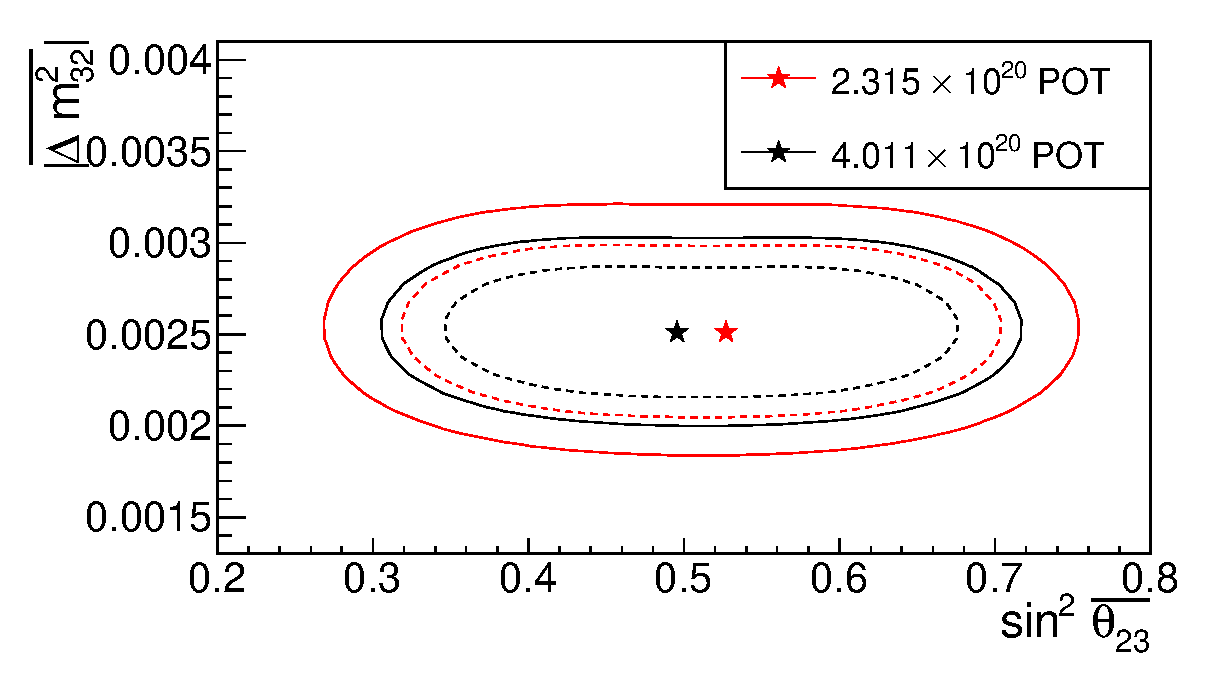
\includegraphics[height=0.37\textheight]{./images/asimov_fit/asimov_comparison_of_different_POT_nh.eps}
\caption {
  Comparison of the 68\% and 90\% Asimov sensitivity regions with the POT up to March 12, and the full Run 6 POT.
  The normal mass hierarchy is assumed.
}
\label{fig:results_asimov_changing_pot_nh}
\end{figure*}

\begin{figure*}[htb]
\center
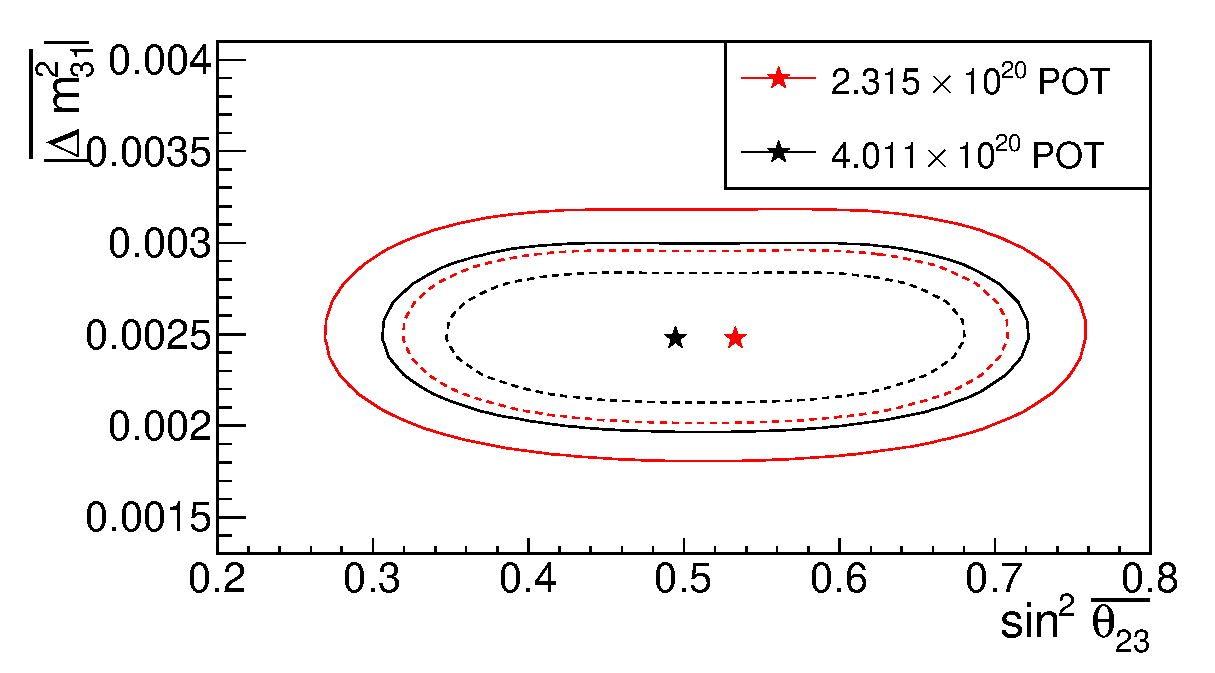
\includegraphics[height=0.37\textheight]{./images/asimov_fit/asimov_comparison_of_different_POT_ih.eps}
\caption {
  Comparison of the 68\% and 90\% Asimov sensitivity regions with the POT up to March 12, and the full Run 6 POT.
  The inverted mass hierarchy is assumed.
}
\label{fig:results_asimov_changing_pot_ih}
\end{figure*}

\begin{figure*}[htb]
\center
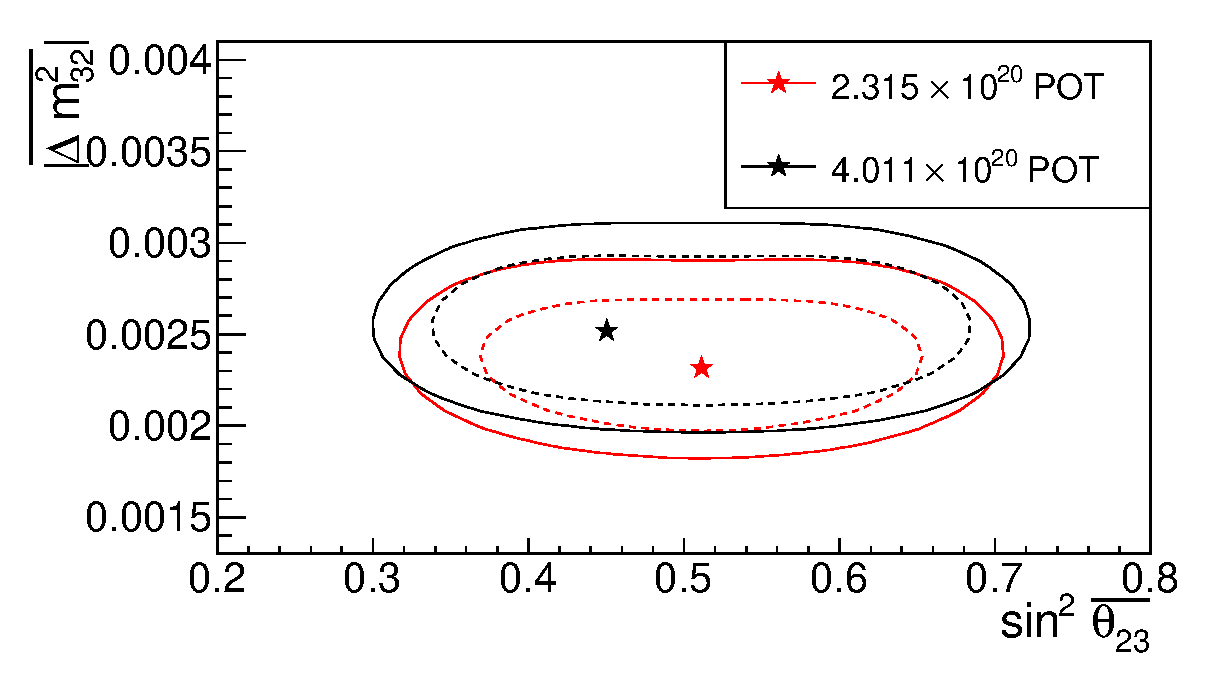
\includegraphics[height=0.4\textheight]{./images/data_fit/comparison_of_different_POT_nh.eps}
\caption {
  Comparison of the 68\% and 90\% confidence regions with the data up to March 12, and the full Run 6 POT.
  The normal mass hierarchy is assumed.
}
\label{fig:results_data_changing_pot_nh}
\end{figure*}

\begin{figure*}[htb]
\center
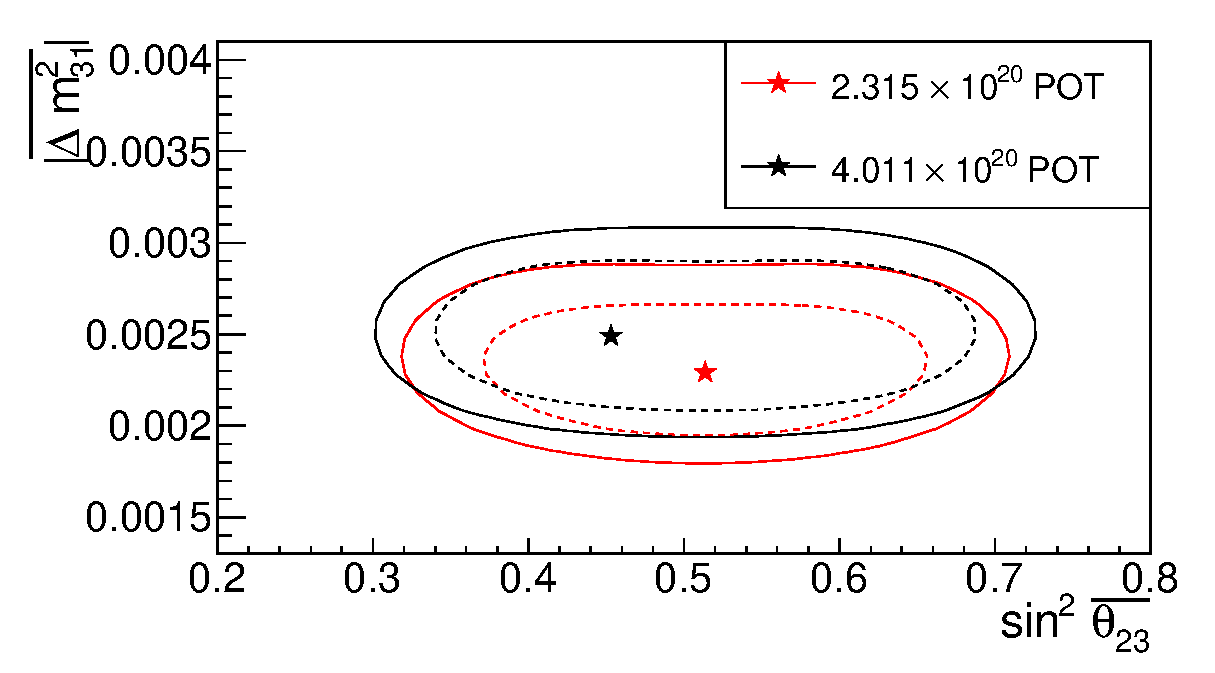
\includegraphics[height=0.4\textheight]{./images/data_fit/comparison_of_different_POT_ih.eps}
\caption {
  Comparison of the 68\% and 90\% confidence regions with the data up to March 12, and the full Run 6 POT.
  The inverted mass hierarchy is assumed.
}
\label{fig:results_data_changing_pot_ih}
\end{figure*}

\begin{figure*}[htb]
\center
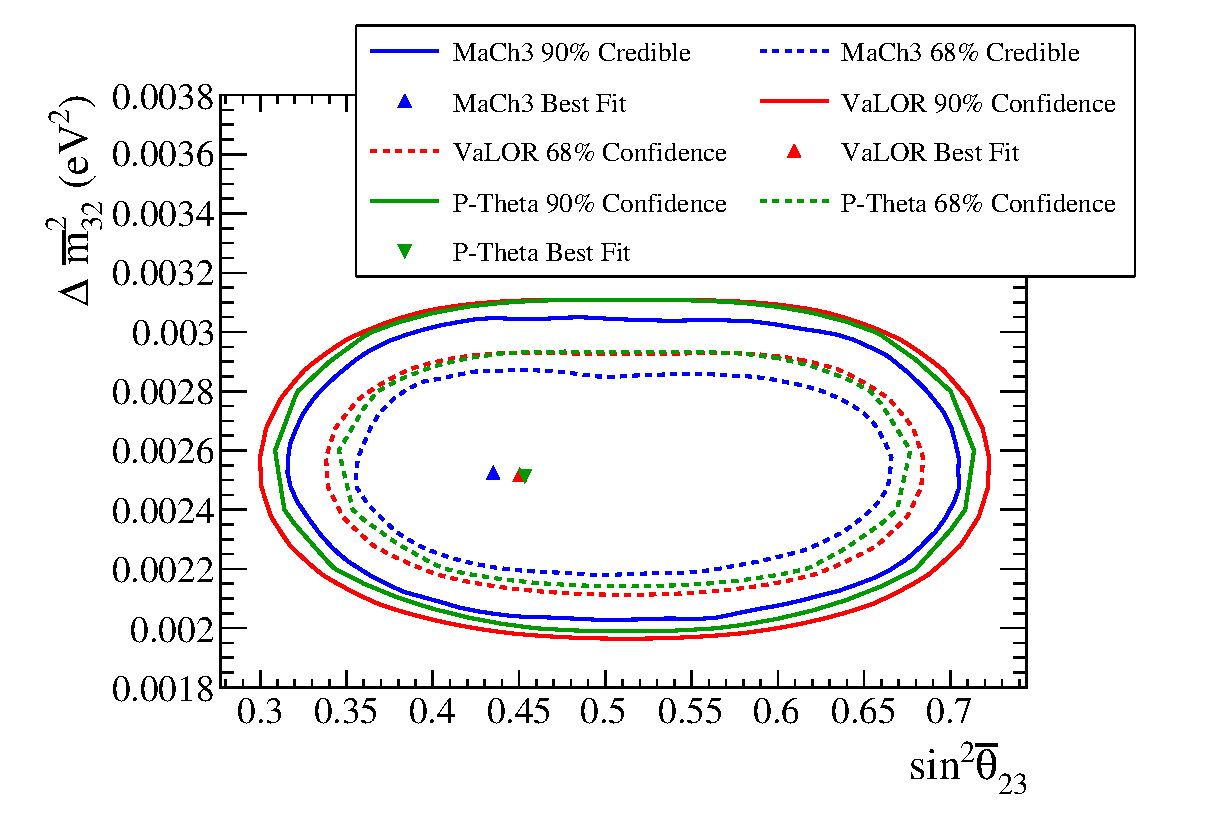
\includegraphics[height=0.4\textheight]{./images/data_fit/compare_threeanalyses.eps}
\caption {
  Confidence regions for the VALOR normal hierarchy fit to the Run 5+6 dataset 
  compared to the other oscillation groups.
  This figure was produced by the MaCh3 group.
}
\label{fig:results_data_contour_groups}
\end{figure*}

\begin{figure*}[htb]
\center
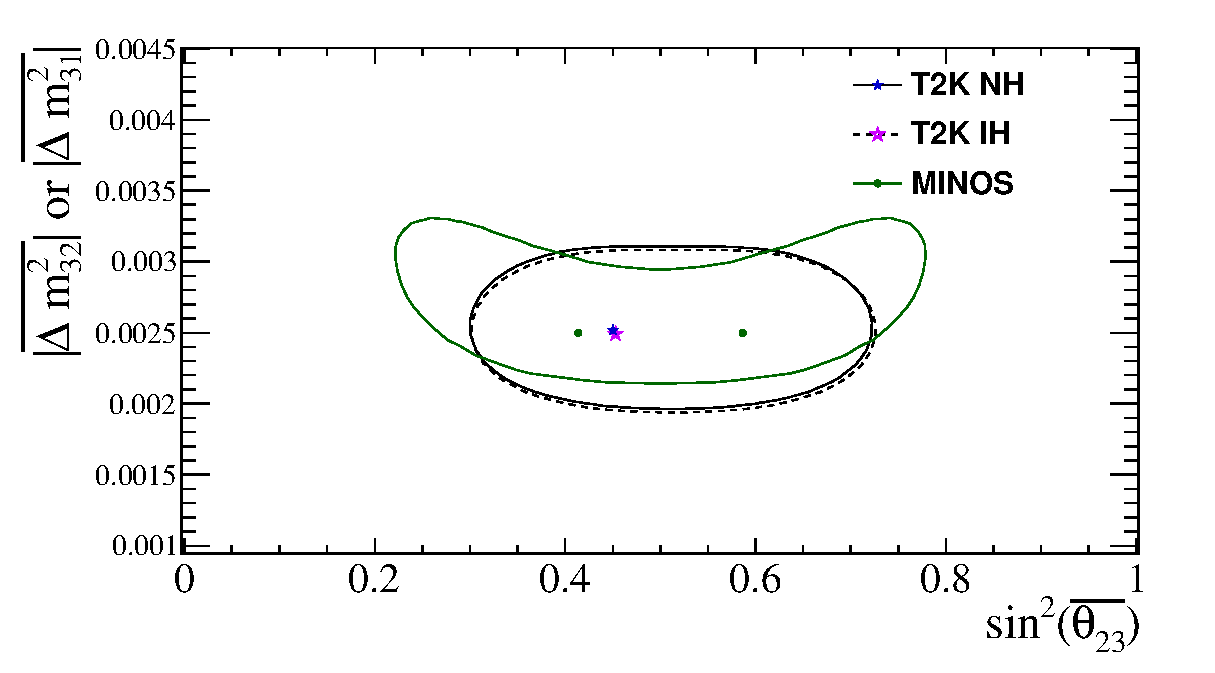
\includegraphics[width=0.9\textwidth]{./images/data_fit/realdata_with_reactor_values_plus_minos.eps}
\caption {
  90\% CL allowed regions,
  constructed with the constant-$\Delta\chi^{2}$ method,
  from the fit to the Run 5+6 dataset,
  with the effects of statistical fluctuations and postfit systematic variations being included.
  The best-fit point for each hypothesis is shown, with the larger point representing the better of the two fits.
  A MINOS contour has been added for comparison\cite{Adamson:2013whj}.
  This MINOS contour was fitted in $\sin^2{2\theta_{23}}$ but has been converted here to $\sin^2{\theta_{23}}$.
}
\label{fig:results_data_contour_minos}
\end{figure*}

\begin{figure*}[htb]
\center
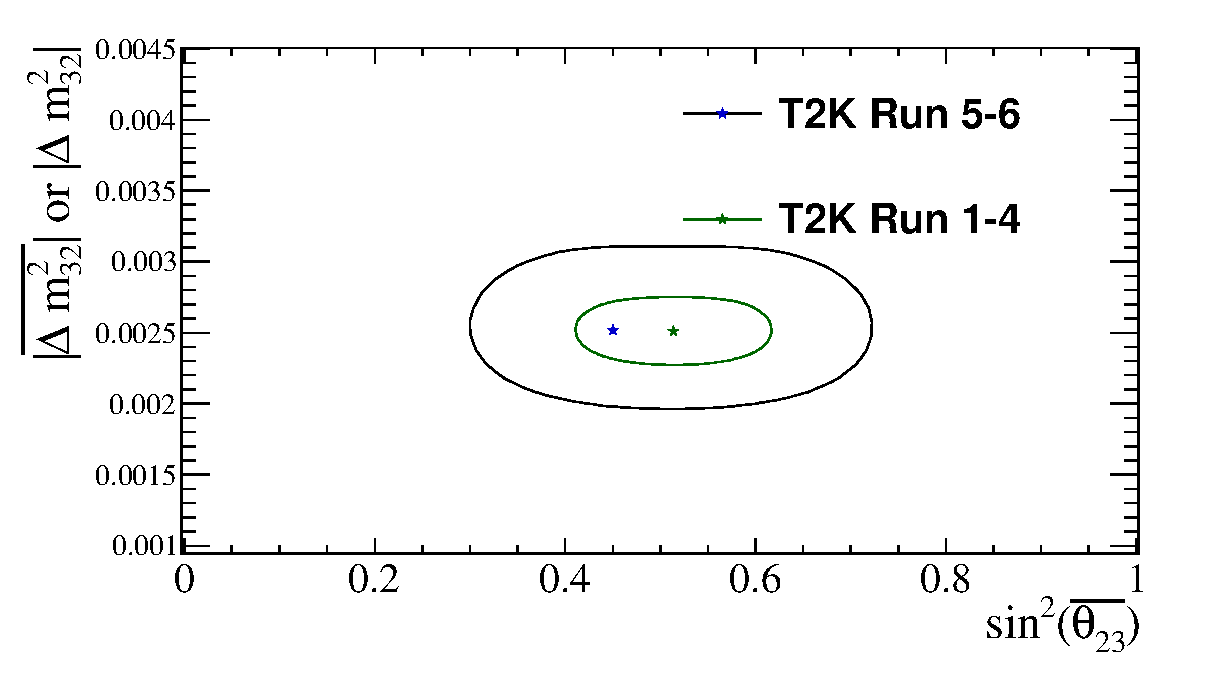
\includegraphics[height=0.37\textheight]{./images/data_fit/realdata_with_reactor_values_plus_kdi.eps}
\caption {
  90\% CL allowed regions,
  constructed with the constant-$\Delta\chi^{2}$ method,
  from the fit to the Run 5+6 dataset,
  with the effects of statistical fluctuations and postfit systematic variations being included.
  The normal hierarchy is assumed, and the official T2K $\nu_\mu$ disappearance contour from the run1-4
  neutrino mode fits was drawn.
}
\label{fig:results_data_contour_kdi}
\end{figure*}

\begin{figure*}[htb]
\center
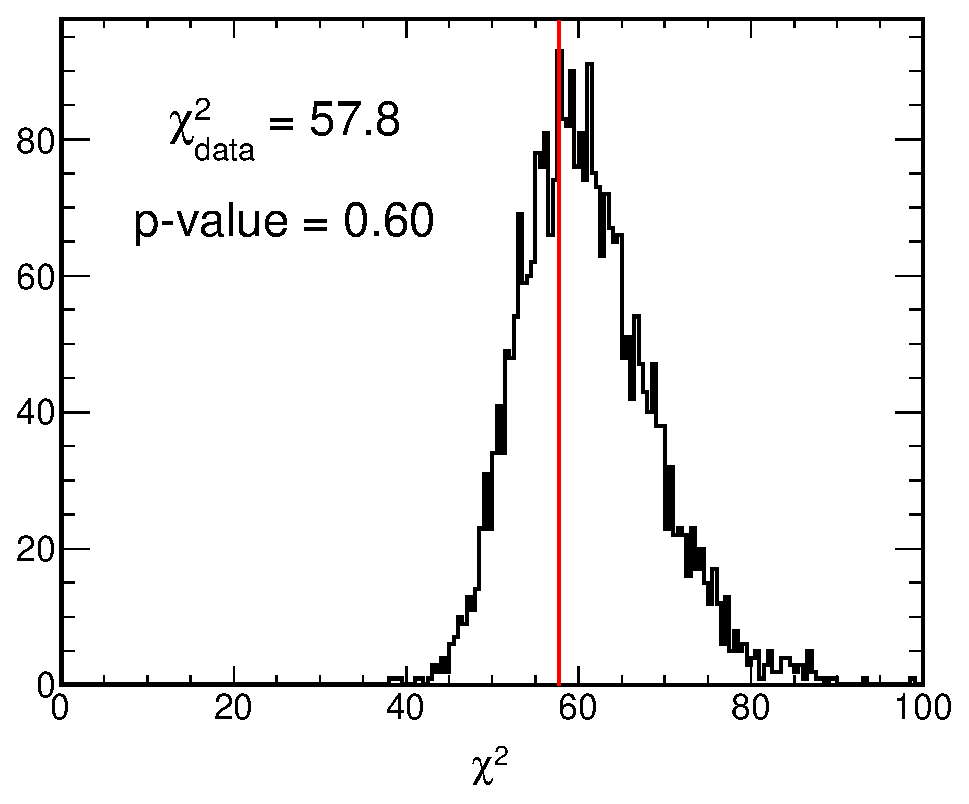
\includegraphics[height=0.37\textheight]{./images/data_fit/chisq_data_numode_bestfit_4.011E20_NH.eps}
\caption {
  Distribution of best-fit $\chi^2$ from 3k toy MC experiments whose true input values of $\sin^{2}\overline{\theta}_{23}$ and 
  $|\overline{\Delta m}^{2}_{32}|$ are equal to the best-fit equivalent parameters for the normal mass hierarchy from the 
  official T2K Run 1-4 result in neutrino beam mode ($\sin^{2}\theta_{23}$ = 0.514, $|\Delta m^{2}_{32}|$ = 
  2.51$\times$10$^{-3}$eV$^{2}$/c$^{4}$). The input values of the other oscillation parameters are given in the normal hierarchy 
  column of Tab.~\ref{tab:osc_params_fixed_values_reactor}. The toy experiments are generated for \TotalPot{} POT and the normal 
  mass hierarchy is assumed. Systematic variations and statistical fluctuations are applied to the toy datasets, and all \NSyst{} 
  systematic parameters are included in the fits. 
  The value of $\chi^2$ from a fit of the \TotalPot{} POT Run 5-6 antineutrino mode data fixing $\sin^{2}\overline{\theta}_{23}$ 
  = 0.514 and $|\overline{\Delta m}^{2}_{32}|$ = 2.51$\times$10$^{-3}$eV$^{2}$/c$^{4}$ (the best-fit equivalent parameters from 
  the Run 1-4 neutrino mode analysis) is shown as a red line.  
}
\label{fig:chisq_data_numode_bestfit_NH}
\end{figure*}
